\begin{figure}[htbp]
	% Partly taken from http://www.texample.net/tikz/examples/convolution-of-two-functions/
	\centering
	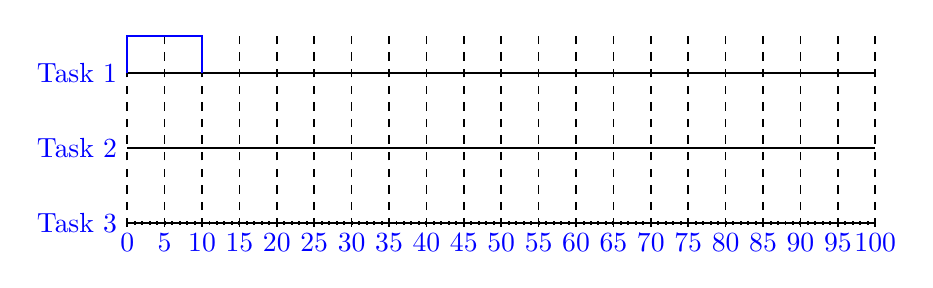
\begin{tikzpicture}[
		scale=0.095,
		line width=0.25mm,
		every node/.style={scale=1, text=blue},
		major tick/.style={semithick, dashed},
		x tick label/.style={anchor=north, minimum width=5mm},
		task1/.style={blue},
		task2/.style={red},
		task3/.style={green},
		desc/.style={anchor=east}
		]
	
	% Task 1
	\draw (0, 0) -- (100, 0);
	\node[desc] at (0, 0) {Task 3};
	
	% Task 2
	\draw (0, 10) -- (100, 10);
	\node[desc] at (0, 10) {Task 2};	
	
	% Task 3
	\draw (0, 20) -- (100, 20);
	\node[desc] at (0, 20) {Task 1};	
	
	% Small ticks
	\foreach \x in {0, 1,...,100}{
		\draw (\x, -0.25) -- (\x, 0.25);
	}
	
	% Major ticks with label
	\foreach \x/\label in {0, 5,...,100}{
		\node[x tick label] at (\x, 0) {$\label$}; 		
		\draw[major tick] (\x, -0.5) -- (\x, 26);
	}
	
	\draw[task1] (0, 20) -- (0, 25) -- (10, 25) -- (10, 20);
	%\draw[task2] (10, 10) -- (10, 15) -- (20, 15) -- (20, 10);
	%\draw[task3] (20, 0) -- (20, 5) -- (30, 5) -- (30, 0);
		
	\end{tikzpicture}
%	\caption{Ablaufübersicht}
\end{figure} 